\documentclass{imcs}
\usepackage[T2A]{fontenc}
\usepackage[utf8x]{inputenc}
\usepackage[russian]{babel}
\usepackage{graphicx}
\usepackage{hyperref}
\usepackage{enumitem}
\usepackage{listings}
\usepackage{courier}
\usepackage{titlesec}
\usepackage{lscape}


\titleformat*{\section}{\LARGE\bfseries\sffamily}
\titleformat*{\subsection}{\Large\bfseries\sffamily}
\titleformat*{\subsubsection}{\large\bfseries\sffamily}
\titleformat*{\paragraph}{\large\bfseries\sffamily}
\titleformat*{\subparagraph}{\large\bfseries\sffamily}

\lstset{basicstyle=\footnotesize\ttfamily,breaklines=true}



\makeatletter
\let\old@itemize=\itemize
\def\itemize{\old@itemize
\setlength{\itemsep}{10pt}
\setlength{\parskip}{0pt}
\setlength{\leftskip}{0pt}
}
\makeatother

\makeatletter
\let\old@enumerate=\enumerate
\def\enumerate{\old@enumerate
\setlength{\itemsep}{10pt}
\setlength{\parskip}{0pt}
\setlength{\leftskip}{0pt}
}\makeatother

\title{Модуль контролируемого исполнения программ Spawner}
\author{Храпченков Пётр Фёдорович}
\mentorinfo{старший преподаватель}
\mentorname{А.С.~Кленин}
\year{2014}


\begin{document}
\maketitle

\tableofcontents
\pagebreak

\section*{Аннотация}
\addcontentsline{toc}{section}{Аннотация}
Модуль Spawner является частью автоматической проверяющей системы CATS и используется для запуска программ с ограничениями на использование системных ресурсов и получения информации об использованных системных ресурсов программой, а так же информации о ходе исполнения.

Рассмотрены подходы к решению проблемы и осуществлена реализация.

\pagebreak

\section{Введение}
\subsection{Глоссарий}

Системные ресурсы -- Набор системных ресурсов включает в себя время исполнения программы в пользовательском режиме, физическое время исполнения, объем выделенной памяти, объем записанной на диск информации.

Физическое время исполнения -- абсолютное время, определяемое глобальным системным таймером.

Уровень загрузки -- величина, отображающая отношение времени в пользовательском режиме к физическому времени.

Время простоя -- время, в течении которого уровень загрузки программы находился не выше установленного минимального.

Sandboxing -- в компьютерной безопасности защитный механизм для изолированного исполнения программ. Часто используется для запуска непроверенного кода или сомнительных программ от неизвестных разработчиков, поставщиков, подозрительных пользователей или веб сайтов.

JOB\_OBJECT -- это объект, способный иметь имя, настройки безопасности, который контролирует атрибуты ассоциированных с ними процессов. Операции, применяемые к ним, влияют на все процессы, включенные в него. Так, например можно ограничить память, приоритет процессов, а так же завершить их все.


\subsection{Описание предметной области}

На сегодняшний день в России и мире проводится множество соревнований по программированию, включая известный командный чемпионат мира по программированию среди студентов высших учебных заведений АСМ (1), а так же олимпиады школьников по информатике. Обычно при подготовке подобных соревнований разрабатываются пакеты заданий, состоящие из формулировки задачи, условий к входным и выходным данным,  набора тестов, а так же эталонного решения. Для проведения соревнования используются различного рода автоматизированные системы, использующий полученные пакеты заданий. Такие системы предоставляют удобный интерфейс: для участников – просмотра и отправки своих решений, для организаторов – создание соревнований, а так же наблюдения за их ходом.
\subsubsection{Автоматическая система проведения соревнований CATS}
\begin{figure}[htb]
\centering
\includegraphics{./img/cats_screenshot.png}
\caption{Веб интерфейс системы}
\label{cats_screenshot}
\end{figure}

В частности, одной из таких систем является автоматическая система проведения соревнований CATS (2). Система разрабатывалась на базе ДВФУ и успешно применялась при проведении различных турниров. Она состоит из веб-интерфейса, базы данных, а так же модуля judge.
Веб интерфейс предоставляет возможность участвовать в доступных турнирах, просматривать задачи, отправлять соответствующие решения, выполненные в разрешенных системой (турниром) средах разработки, следить за ходом их тестирования, следить за ходом турнира и др. Для организаторов, в свою очередь, веб-интерфейс позволяет создавать турниры, добавлять в них задачи, следить за ходом турнира и др.
Связь между веб интерфейсом и модулем judge осуществляется через базу данных. [2] Веб интерфейс и база данных являются кросс-платформенными составляющими системы и могут быть установлены на компьютеры под управлением различных операционных систем.
Модуль judge использует Spawner для исполнения программ участников с контролем безопасности и ограничений на системные ресурсы. Он представляет собой набор скриптовых утилит, который занимается сборкой и тестированием решений участников и последующей отправкой результата в базу данных (подробнее см. раздел Архитектура).
Модуль Spawner разрабатывался как часть системы CATS и имел достаточный для этого функционал. Однако, с появлением новых типов задач, таких как интерактивные (3) в соревнования вроде Всероссийской олимпиады школьников по информатике стала очевидной необходимость расширения модуля. Так же, на базе ДВФУ неоднократно проводились соревнования искусственного интеллекта, где тоже требуется контролируемое исполнение программ участников, что вместе с предыдущим пунктом поставило задачу множественного исполнения. Дополнительно, консольная утилита Spawner оказалась несовместимой с 64 разрядными операционными системами Windows, в силу специфики кода. К тому же, модуль Spawner являясь чистым Windows приложением не позволяет проводить более тесную интеграцию веб-сервера с модулем judge. Можно дополнить, что другие подобные модули реализуют более расширенный функционал, например, по вводу новых ограничений, таких как ограничение на время простоя. А вследствие отсутствия финальной версии исходного кода нет возможности проводить дальнейшие изменения и улучшения.
Таким образом, перечисленные выше пункты послужили мотивацией к написанию данной работы.

\subsection{Неформальная постановка задачи}

Требуется доработать модуль Spawner для выполнения следующих требований:
Полная совместимость с предыдущей версией Spawner’а для внедрения в систему CATS.
Проверка на наличие и корректная обработка исключений, возникших во время работы программы.
Борьба с гуи исключениями
Ограничения на использование подконтрольной программой системных ресурсов:
память
время работы
время исполнения
запись в файлы
время простоя
Вывод отчета в других форматах, включая как json, так и форматы отчетов других подобных модулей
Кроссплатформенность
Возможность работы системы как в 32 так и в 64 битном окружении системы Windows.
Дальнейшая разработка совместимых версий для Linux и др.
Работа со стандартными потоками - stdin, stdout и stderr, их перенаправление
Корректный запуск программ из-под заданного пользователя.
Множественное исполнение программ
Перенаправление потоков ввода вывода
Поддержка ролей запускаемых процессов
Поддержка ролей запускаемых процессов
Анализ и дополнение существующего формата входных аргументов, соответствующего указанным выше требованиям
Интеграция доработок в систему CATS
Возможность отдельного использования функционала утилиты в виде библиотеки.


\subsection{Обзор существующих методов решения}

\subsubsection{Аналогичные решения}

Следующие системы тестирования включают в себя модули подобные реализуемому в данном проекте spawner’у
ejudge http://ejudge.ru/   
ejudge - это система для проведения различных мероприятий, в которых необходима автоматическая проверка программ. Система может применяться для проведения олимпиад,
поддержки учебных курсов и т.д.
Для контроля исполнения используется патч к ядру Linux. Модуль контроля исполнения программ представляет собой набор скриптов. Невозможно портирование скриптов на ОС Windows в силу их зависимости от системных функций.
PCMS2/Run http://neerc.ifmo.ru/trains/information/software.html
PCMS2(Programming Contest Management System)
Система контроля исполнения представляет собой консольную утилиту. Используется динамическая библиотека. Для создания и контроля исполнения процесса от другого пользователя требуются особые привилегии.
Во многом схожий проект, однако для запуска программ постоянно используется режим отладки.
Contester
Contester - это система для проведения турниров и индивидуального решения задач по олимпиадному программированию (спортивному программированию). Система содержит условия задач - от легких до олимпиадных - и возможность проверки решений на большинстве современных языков: C++, Object Pascal, Java и языках .NET: C\#, J\# и Visual Basic.
Не тестировалось.
Executor http://acmtest.ru/
Executor - автоматизированная сетевая тестирующая система для проведения турниров по программированию по правилам ACM. Executor - freeware, распространяется бесплатно и без каких-либо ограничений на использование.
Тестирование контроля исполнения не производилось
PC² http://www.ecs.csus.edu/pc2/
PC²(Programming Contest Control System) - система разработанная в Калифорнийском Государственном Университете Sacramento (CSUS) в поддержку соревнований по программированию, проводимых ACM и, в частности, ACM International Collegiate Programming Contest (ICPC) и его региональных этапов. 
Контроль исполнения, как неотъемлемая часть общей системы.
olympiads.ru/RUN http://olympiads.ru/school/system/index.shtml
Система самотестирования olympiads.ru. Используется для тестирования решений задач, представленных на соответствующем сайте. Система работает на платформе Windows, имеет инсталляционную программу и документацию. 
Вследствие того что система не поддерживается с 2003 года и имеет узкий функционал в рамках данной работы детально рассматриваться не будет.
DOMjudge http://domjudge.sourceforge.net/
DOMjudge - автоматизированная тестирующая система, для проведения соревнований по программированию, подобных ACM ICPC. Основной упор сделан на удобство использования и безопасность. Система участвовала во многих соревнованиях, распространяется свободно на условиях открытого ПО. 
Для контроля исполнения используется набор небольших консольных утилит.
dudge http://code.google.com/p/dudge/
Dudge - это универсальная система для проведения олимпиад по программированию и другим предметам, написанная на Java и J2EE с использованием СУБД PostgresSQL и распространяющаяся по лицензии GPL. 
В качестве контроля исполнения используется динамическая библиотека, реализована для Windows и Unix. Библиотека используется в Java коде. Для создания и контроля исполнения процесса от другого пользователя требуются особые привилегии.(не подтверждено)
cats-judge/Spawner прототип http://imcs.dvgu.ru/cats/docs/spawner.html
cats-judge - автоматизированная тестирующая система, для проведения как одиночных, так и командных соревнований по программированию.
Для контроля исполнения используется консольная утилита. Создание и контроль исполнения процесса от другого пользователя требуют особые привилегии.
Spawner http://code.google.com/p/spawner/
Дальнейшее развитие модуля контроля запуска и исполнения программ cats-judge/Spawner .
На данный момент представляет собой обратно совместимую консольную утилиту с расширенными, по сравнению с предыдущей версией, возможностями.
Функционал реализован только для систем семейства Windows.

\begin{landscape}
\begin{table}[h!]
\begin{center}
\begin{tabular}{|l|c|c|c|c|c|c|}
\hline
  Название   &  Операционная  &  Лицензия  &  Интерфейс  &  Язык	 		&  Защищенный запуск 	  & Комментарий \\
         	&  система    	 &      		  &  	   		&  реализации   	& под другим пользователем &	           \\
\hline
 Perl    &  +          &  +/-        &             &  +          &  +   &   -    \\
\hline
\end{tabular}
\caption{Поддержка замыканий и анонимных функций современными ЯП}\label{tab:wsi_diff_rel}
\end{center}
\end{table}
\end{landscape}


\subsubsection{Описание предшествующих работ}
Студенты нашей кафедры успешно развивали компилятор Fpc в рамках своих
курсовых и дипломных работ:
\begin{enumerate}
    \item Дипломная работа «Расширение компилятора Free Pascal для поддержки обобщённого программирования». Автор Нелепа А.А. Руководитель Кленин А. С. 2007г.\cite{diplomnelepa}
    \item Курсовая работа «Анализ потоков управления для языка программирования Pascal» Автор Баль Н.В. Руководитель Кленин А.С. 2008г.\cite{coursebal}
    \item Курсовая работа «Доработка компилятора Free Pascal: case of string» Автор Денисенко М.В. Руководитель Кленин А.С. 2009г.\cite{misha}
    \item Курсовая работа «Оператор for-in для компилятора Free Pascal» Автор Лукащук М.А. Руководитель Кленин А.С. 2010г.\cite{courseluck}
\end{enumerate}

\subsubsection{Вывод}

Ценность замыканий подтверждена их популярностью и востребованностью. 
Сегодня замыкания поддерживают большинство языков программирования, а программисты 
активно используют их на практике. Поэтому для поддержания компилятора FPC в 
актуальном состоянии необходимо реализовать в нём поддержку замыканий.

\subsection{План работ}

\begin{enumerate}
    \item Согласовать работу с разработчиками FPC.
    \item Изучить архитектуру и исходных код компилятора.
    \item Изучить реализацию замыканий в похожих языках программирования.
    \item Спроектировать реализацию.
    \item Поэтапно осуществить реализацию:
      \begin{itemize}
          \item Добавить возможность объявлять анонимные функции. Запретить захват переменных.
          \item Добавить возможность захвата переменных функции, объявляющей замыкание.
          \item Добавить возможность захвата любых локальных переменных, 
                доступных в текущем лексическом контексте\footnote{За исключением случаев, описанных в разделе "Функциональные требования".}.
      \end{itemize}        
\end{enumerate}

\section{Требования к окружению}

\subsection{Требования к аппаратному обеспечению}

Для работы требуется компьютер, пригодный для компиляции исходного кода программы или исполнения существующих пакетов.
Т.е. кроме работающих процессора, оперативной и постоянной памяти требуются
клавиатура и монитор.

\subsection{Требования к программному обеспечению}

\subsubsection{Операционная система}
\begin{itemize}
    \item Windows не ниже ХР
    \item Linux
\end{itemize}

\subsubsection{Компилятор} 
\begin{itemize}
    \item Microsoft Visual Studio 2005 и новее или G++ 4.7.7 и новее
    \item CMake 2.6 и новее
\end{itemize}
    
\subsection{Требования к пользователям}
Программисты, владеющие языком программирования Free Pascal или Delphi.

\section{Архитектура системы}

Несмотря на то, что для конечного пользователя автоматизированная система представлена в виде Web интерфейса, она является аппаратно-програмным комплексом, состоящим из нескольких модулей.
В рамках данной работы необходимо рассмотреть внутреннее устройство системы, для обоснования некоторых принятых решений.
\iffalse TODO: каких? \fi

\subsection{Архитектура системы CATS}
Автоматизированная система CATS состоит из нескольких частей: веб интерфейс, база данных, а так же модуль judge. 


\subsubsection{Веб интерфейс}

\subsubsection{База данных}
В базе данных системы хранятся данные о проводимых турнирах, пакеты задач, информацию об участниках, их попытках, а так же информация по средам разработки.


\begin{figure}[htb]
\centering
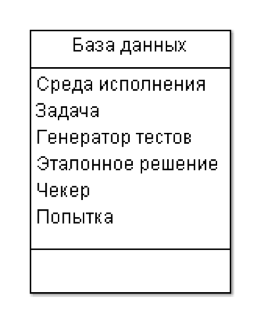
\includegraphics{./img/db.png}
\caption{Схематичное изображение базы данных}
\label{dbfields}
\end{figure}

\subsubsection{Модуль judge}
Модуль judge в свою очередь содержит загруженный кэш задач, кэш попыток, различные конфигурационные файлы и модуль Spawner.

\begin{figure}[htb]
\centering
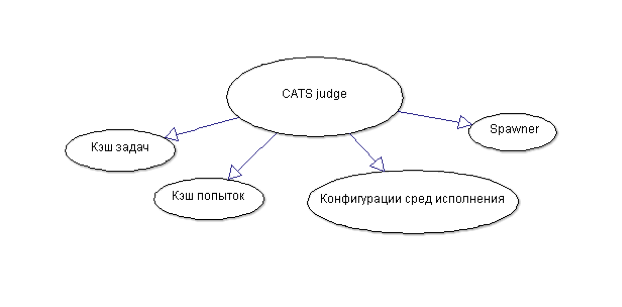
\includegraphics{./img/judge.png}
\caption{Схематичное устройство модуля judge}
\label{judgemodule}
\end{figure}

В общем случае коммуникация между модулями проходит в следующем порядке:

\begin{figure}[htb]
\centering
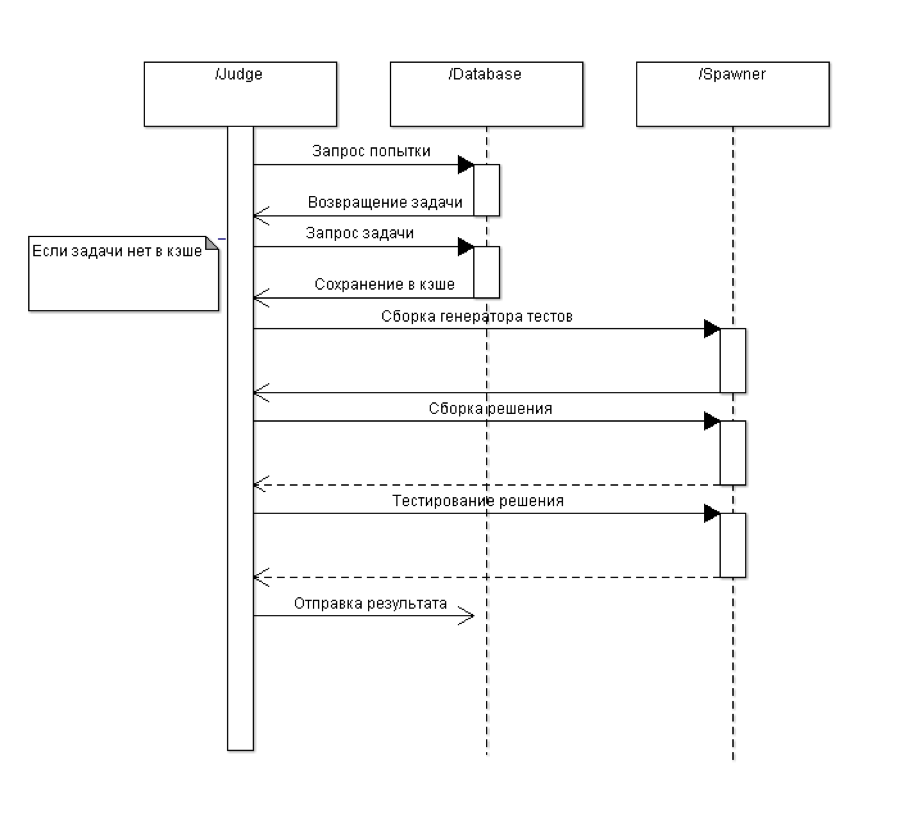
\includegraphics{./img/judgeinteraction.png}
\caption{Схема работы модуля judge}
\label{judgeinteraction}
\end{figure}

\subsubsection{Модуль Spawner}

Во время проведения тестирования требуется, чтобы программа не нарушала некоторый установленный правилами соревнований набор ограничений системных ресурсов. Так же в случае некорректного хода исполнения тестируемой программы требуется определить характер и возможную причину ошибок и сообщить об этом организаторам и участникам. Этой работой занимается модуль Spawner.
Являясь подмодулем judge, Spawner в свою очередь разбит на три основных слоя: консольный интерфейс, прослойка совместимости и библиотека.
\begin{figure}[htb]
\centering
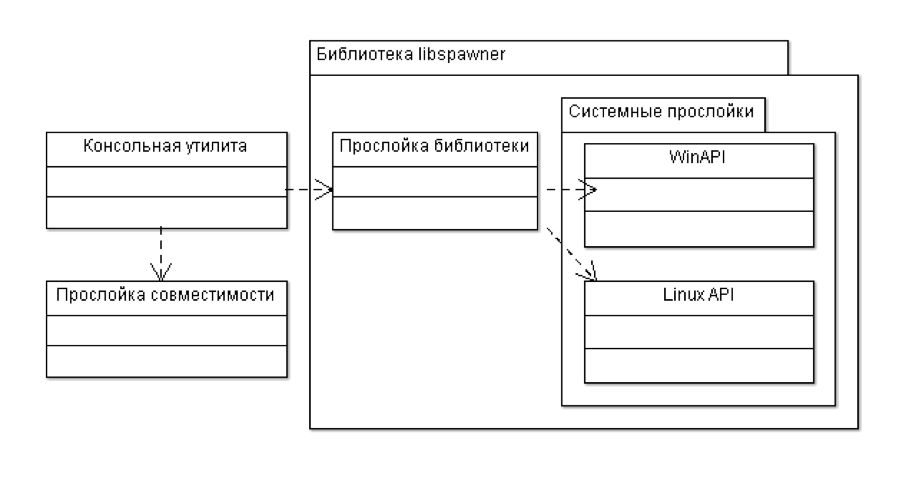
\includegraphics{./img/sp.png}
\caption{Схема устройства модуля Spawner}
\label{spawnermodule}
\end{figure}
Консольная утилита предоставляет интерфейс командной строки пользователю и, в зависимости от режима совместимости, набор аргументов и формат отчета.
Прослойка совместимости выполняет связующую роль выходных данных библиотеки libspawner и требуемого формата отчета/аргументов.
Сама же библиотека представляет абстрактный интерфейс, обеспечивающий доступ к системным функциям.



\pagebreak



\section{Функциональные требования}

Компилятор должен:
\begin{enumerate}
    \item Позволять объявлять анонимные подпрограммы внутри тела других подпрограмм. В том числе с любым уровнем
вложенности. Синтаксис объявления анонимной подпрограммы такой же как и для обычной подпрограммы, с двумя
исключениями:
        \begin{itemize}
            \item после ключевых слов procedure и function нет идентификатора, а сразу идет опциональный список формальных аргументов;
            \item после списка формальных аргументов (если он опущен, то после ключевых слов procedure или function) не ставится точка с запятой.
        \end{itemize}

         Пример 1:
\begin{lstlisting}
  procedure begin
    Writeln('inside');
  end;
\end{lstlisting}

         Пример 2:
\begin{lstlisting}
  procedure begin
    Writeln('inside');
  end;
\end{lstlisting}

    \item Позволять анонимным функциям возвращать значения, используя ключевое слово Result:

Пример:
\begin{lstlisting}
  function(num: Integer): Integer begin
    Result := num + 10;
  end;
\end{lstlisting}

    \item Запрещать анонимным процедурам использовать переменную Result объемлющей функции:

Пример:
\begin{lstlisting}
  function Calculate: Integer;
  begin
    ...
    procedure begin
      Result := 10; // Error, result can't be captured
    end;
  end;
\end{lstlisting}

    \item Запрещать анонимным процедурам использовать параметры объемлющей функции, объявленные с модификатором
var или out.

\iffalse TODO: улучшить \fi

    \item Запрещать анонимным процедурам использовать переменные, объявленных в обработчике исключений.

\iffalse TODO: улучшить \fi

    \item Позволять анонимным процедурам использовать переменные, объявленные в объемлющей функции:

Пример:
\begin{lstlisting}
  procedure Calculate: Integer;
  var num: Integer;
  begin
    ...
    procedure begin
      num := 10;
    end;
  end;
\end{lstlisting}

    \item Позволять анонимным процедурам использовать переменные, объявленные в объемлющей функции, при уровне вложенности больше 1:

Пример:
\begin{lstlisting}
  procedure Outer;
  var num: Integer;
    procedure Calculate;
    begin
      ...
      procedure begin
        num := 10;
      end;
    end;
  begin
   ...
\end{lstlisting}

    \item Продлевать время жизни захваченных переменных. Время жизни захваченной переменной определяется не временем работы функции, где она объявлена, а временем жизни всех ссылающихся на неё замыканий.

    \item Управлять памятью замыканий автоматически, используя счётчик ссылок. Время жизни замыкания заканчивается
 только, когда не остаётся указателей соответствующего типа, ссылающихся на это замыкание.
      
    \item Осуществлять захват переменных по ссылке. Замыкания, созданные в одном лексическом контексте должны иметь доступ к одним и тем же переменным.
      
    \item Корректно осуществлять проверку типов в момент присваивания значений переменным-указателям на замыкание. Это значит, что:
        \begin{itemize}
            \item Переменной можно присваивать определение анонимной функции, если сигнатура анонимной функции
совпадает с сигнатурой, указанной в определении типа переменной. Другими словами, в этом случае используется
структурная эквивалентность выражений, т.к. определение анонимной функции не содержит имя типа.
            \item Переменной можно присваивать значение другой переменной, только если имена типов этих переменных
совпадают. Т.е. в этом случае используется именная эквивалентность выражений.
        \end{itemize}

\iffalse TODO: примерчики \fi
        
      \item Корректно осуществлять проверку типов, если замыкание определено в качестве фактического параметра.
В этом случае так же используется структурная эквивалентность выражений, т.к. определение анонимной функции не
содержит имя типа.

\iffalse TODO: примерчики \fi
        
    \item Предоставлять для вызова замыкания синтаксис аналогичный синтаксису вызова обычных указателей
 на функцию:
        \begin{itemize}
          \item Если замыкание имеет непустой список аргументов, то для вызова в имени переменной-указателя
в круглых скобках добавляется список фактических параметров, разделённых запятыми.
          \item Если замыкание имеет пустой список параметров, то в выражении, состоящем только из вызова
замыкания круглые скобки не содержащие аргументов можно опустить.

\iffalse TODO: примерчики \fi
        \end{itemize}
        
  \item Корректно осуществлять проверку типов во время вызова замыкания. Это значит, что:
        \begin{itemize}
          \item Количество фактических параметров должно равняться количеству формальных параметров.
          \item Типы фактических параметров должны быть эквивалентны типам формальных параметров.
        \end{itemize}

    
\end{enumerate}


\section{Требования к интерфейсу}

Весь функционал к модулю Spawner должен быть доступен через интерфейс командной строки. Параметры по умолчанию должны быть загружены из переменных окружающей среды. По окончанию исполнения программа должна выдавать отчет. Должна присутствовать возможность сохранения отчета в отдельный файл. Так же для удобства должна присутствовать возможность вывода стандартных потоков в консоль или файл(по выбору). К тому же должна присутствовать возможность запуска программы из-под пользователя с заданным именем и паролем. И наконец, должна быть реализована простейшая система перевода единиц, благодаря которой было бы возможно передавать программе ограничения в разных форматах. Дополнительно требуется возможность для соединения потоков ввода/вывода разных процессов с помощью консольных аргументов.

Требуется реализовать удобный интерфейс программной библиотеки для использования возможностей контролируемого исполнения в других проектах.

Так же необходимо исследовать другие аналогичные системы автоматизированные системы соревнований и предложить интерфейс, упрощающий написание соответствующих прослоек совместимости для возможного в них внедрения модуля Spawner. Например, системы, у которых аналогичные модули представлены зависимыми от операционной системы программами, могут быть портированы с помощью замены системнозависимого модуля на Spawner.

Запуск контроля исполнения программ должен осуществляться следующим способом

sp.exe [ограничения и опции] программа[ аргументы программы]
Пример использования:

\begin{lstlisting}
sp.exe -tl=400ms -wl=1 -ml=1 tests/write-limit/write-limit.exe
\end{lstlisting}

Пример отчета можно посмотреть в соответствующем разделе.

\section{Проект}

\subsection{Средства реализации}

При анализе задачи ставился акцент на следующие моменты
\begin{itemize}
	\item	переносимость проекта на другие операционные системы
	\item	гибкая настройка проекта
	\item	интеграция с системой тестирования
	\item	удобная система объектов и модулей
\end{itemize}
В следствие чего был выбран язык реализации С++ и система сборки CMake. Для реализации системы тестирования использовался CMake, CTest и Python.
Describe link with CATS


\subsection{Структуры данных}

Основным классом можно назвать класс runner, а так же его потомок – secure\_runner.
Он отвечает за создание процесса с определенными настройками и дальнейший контроль исполнения. Этому классу передаются опции и ограничения, а так же настройки перенаправления потоков ввода/вывода.
Опции представляют собой класс options\_class, полями которого являются настройки исполнения.
Ограничения представляют собой класс restrictions\_class.


\subsection{Модули и алгоритмы}

Spawner, являясь модулем автоматизированной системы CATS, в свою очередь разделен на несколько подмодулей — статическая библиотека libspawner, сам spawner или sp, представляющий из себя консольную утилиту, а так же модуль совместимости. Помимо этого в проекте содержится модуль тестирования.

\subsubsection{Библиотека libspawner}

Исходные файлы библиотеки располагаются в соответствующей директории.
В папке inc - содержатся заголовочные файлы. В корне директории находится файл spawner.h, который является основным, для включения в какой-либо проект.
Содержимое папки inc
buffer.h – модуль отвечающий за конечные точки перенаправленных потоков ввода/вывода
compatibility.h – модуль отвечающий за совместимость со старой версией Spawner'а
delegate.h – модуль отвечающий за делегированный запуск процессов
error.h – модуль отвечающий за обработку ошибок системы Spawner а так же дальнейший их вывод
options.h - модуль отвечающий за класс настроек
pipes.h - модуль отвечающий за перенаправление потоков ввода/вывода
platform.h - модуль отвечающий за системно зависимые переменные и типы
report.h - модуль для получения строковых значений из перечислимых типов проекта
restrictions.h - модуль класса ограничений
runner.h – модуль содержащий базовый и минимальный класс, способный запускать программы
securerunner.h – модуль отвечающий за ограниченный запуск программ
session.h – модуль отвечающий за уникальность сессии делегированного запуска
status.h - модуль статусов
uconvert.h - модуль преобразования единиц, созданный для повышения комфорта работы с программой
В папке src, в корне или в соответствующей операционной системе директории содержатся реализации соответствующих классов.

Используя набор предоставляемых классов и интерфейсов, можно создавать множество процессов и, контролируя их исполнение, обеспечивать их взаимосвязь друг с другом.
В качестве примера был создан демонстрационный проект(см. материалы в конце), представляющий из себя игру с угадыванием последовательности чисел. После того как программно задаются участники – некоторые исполняемые файлы, программа-исполнитель загадывает последовательность чисел и на догадки программ-участников отвечает сколько из чисел угаданы верно. Игра продолжается, до тех пор, пока все участники не угадают загаданную последовательность чисел. Коммуникация между игроками и исполнителем осуществляется через потоки ввода/вывода, соединенные друг с другом программно, с помощью средств libspawner, а так же подобная программа была реализована с использованием консольного интерфейса Spawner'а.

\subsubsection{Модуль консольной утилиты}

Проект включает в себя статическую библиотеку libspawner.
Состоит из двух внутренних модулей - модуль парсинга консольных аргументов SimpleOpt и главный модуль, использующий интерфейсы libspawner для реализации поставленной темой задачи.

\subsubsection{Модуль совместимости}
Представляет собой прослойку, позволяющую структуры данных получаемых от библиотеки переводить в различные форматы соответствующие 
\subsubsection{Модуль тестирования}
Содержит набор тестов. Подробнее смотри раздел «Реализация и тестирование».
\subsubsection{Механизм ограничения}
В новой реализации Spawner унаследовал способ наложения ограничений на дочерние процессы. Для этого используется используется механизм JOB\_OBJECT'ов [2], позволяющий на уровне системы контролировать использование системных ресурсов программой, которой был назначен этот объект. В случае превышения конкретного ресурса, можно определить что это был за ресурс и каково было его использование. На некоторые ресурсы ограничения можно накладывать непосредственно. Ресурсы для которых такой возможности нет предлагается наблюдать в отдельном потоке Spawner'а, и, в случае нарушения, завершать JOB\_OBJECT c указанным кодом.

\subsubsection{Механизм перенаправления потоков ввода/вывода}
В данной работе использовался подход, сходный с реализованным в оригинальной версии Spawner'а. Был реализован гибкий интерфейс классов, построенный поверх системной прослойки для осуществления таких схем как «один  источник – много выходов». Интерфейс классов представлен двумя базовыми объектами – соединительный канал (pipe) (4) и буфер данных. Соединительный канал осуществляет связь между соответствующим потоком ввода/вывода дочернего процесса и буфером. Буфер данных представляет собой абстрактный объект, который может осуществлять как запись/чтение файла, консоли, так и работу с участками памяти. Т.е. данные из соединительного канала с помощью объекта буфера могут быть выведены в совершенно различные источники. Каждый объект соединительного канала имеет свой отдельный программный поток, в котором в зависимости от направления канала происходит чтение из буферов и запись или наоборот, чтение из канала и запись в объекты буферов.

\subsubsection{Отключение диалогов об ошибках и пользовательского интерфейса}
Одним из требований к модули была возможность отключение сообщений об ошибках, выдаваемых как средой разработки так и операционной системой. Для решения проблемы были использованные специальные функции WinAPI, такие как SetErrorMode, а так же были установлены специальные параметры при создании дочерних процессов.
Возможность скрытия графического интерфейса также реализуется при помощи создания процесса со специальными параметрами STARTF\_USESHOWWINDOW и SW\_HIDE.
Среда разработки Microsoft Visual Studio при компиляции программ в режиме отладки в случае исключения генерирует диалог об ошибке, которые невозможно скрыть ни одним из указанных выше методом. Для решения этой проблемы использовался запуск дочернего процесса в режиме отладки и постоянная проверка на исключение. Когда оно возникает Spawner просто завершает дочерний процесс.

\subsubsection{Запуск программ от другого пользователя}
В изначально версии Spawner'а, а так же в некоторых других подобных модулях для запуска процесса от учетной записи другого пользователя использовалась стандартная функция WinAPI CreateProcessWithLogon. Однако, при выполнении этой функции для дочернего процесса автоматически создается анонимный JOB\_OBJECT. Таким образом, в следствие невозможности назначения нескольких таких объектов одной программе получается, что установление ограничений не представляется возможным. В рамках данной работы было проведено исследование и выделено несколько возможных путей решения.
Первый путь решения предполагает собой написания драйвера ядра с использованием недокументированного API (5). В низкоуровневом системном Windows Driver API существует функция ObReferenceObjectByHandle, позволяющая получить доступ ко всем дескрипторам выбранного процесса. Однако, сложность данного решения заключается как в написании подобного драйвера ядра, так и портировании его на другие системы.
Другим решением является запуск процесса-агента. Однако данное решение было признано неподходящим, вследствие необходимости запуска сервиса-агента, постоянно запущенной пользовательской сессии, а так же сложностями с контролируемым исполнением.
Еще одним решением является делегированный запуск. Делегированный запуск представляет собой запуск дочерним процессом еще одного Spawner'а от учетной записи другого пользователя. Этому процессу «делегируется» роль исполнения конечной программы. Ограничения по системным ресурсам создаются в именном объекте JOB\_OBJECT в главном процессе Spawner'а. В роли имени JOB\_OBJECT'а выступает некоторый идентификатор, получаемый исходя из следующих пунктов:
•	Время запуска родительского процесса Spawner'a
•	Опции запуска дочернего процесса
•	Порядковый номер в случае множественного исполнения
Полученный идентификатор передаются делегату с помощью внутреннего аргумента --session=<id>.
Однако существует сложность наследования дочерними процессами родительского JOB\_OBJECT'а. Эта сложность решается недокументированным поведением API. Для этого родительскому Spawner'у назначается JOB\_OBJECT с параметрами, запрещающими выход дочерних процессов из него. После этого при создании дочерних процессов под другим пользователям они не получают свой анонимный JOB\_OBJECT, наследуя вместо этого соответствующий объект JOB\_OBJECT родителя. После Затем в родительском процессе отменяется запрет на выход дочерних процессов из JOB\_OBJECT'а и делегированный процесс уже запускает заданную программу с необходимыми опциями.
В рамках данной работы была реализована система перенаправления потоков ввода/вывода, основанная на именных соединительных каналах. (4) Однако, из-за этого некоторые программы не исполнялись корректно. Поэтому было решено реализовать перенаправления на основе стандартных безымянных каналов. Созданные каналы передаются процессу «делегату» в качестве стандартных потоков ввода/вывода при создании. После чего, процесс «делегат» уже передает эти потоки запускаемому дочернему процессу.
В случае если отключен режим отладки (см. подробнее раздыл о скрывании ошибок), процесс «делегат» завершается. Иначе он работает в качестве отладчика. Здесь возникает проблема нотификации главного процесса о том, что в дочернем процессе произошло исключение. Одним из возможных способов реализации является использование системы сообщений JOB\_OBJECT'а.

\subsubsection{Множественное исполнение}
Благодаря гибкой системе соединительных каналов и буферов (см. соответствующий пункт о перенаправлении потоков ввода/вывода), соединение двух каналов возможно с помощью объекта буфера, работающего с памятью как на чтение так и на запись.

\subsubsection{Ограничение по времени простоя}
В рамках данной работы для совместимости, а так же улучшения было принято решение реализовать ограничение по времени простоя. Подобное ограничение успешно используется на Полуфинальном этапе чемпионата АСМ (1).
Благодаря  этому ограничению можно сэкономить значительное время на уничтожении процессов по факту не выполняющих полезной работы определенное время. Причинами такого поведения программ могут быть: ожидание выполнения операции ввода/вывода, системная операция сна, различные ожидания объектов и пр. Если в старой версии Spawner'а требовалось ждать 10 секунд глобального таймаута, что для 100 тестов является довольно продолжительным, то сейчас подобные ничего не делающие программы могут быть уничтожены за гораздо более короткое время. 
В качестве входных параметров принимается уровень пороговый загрузки, который будет считаться за простой и ограничение на время простоя. Когда уровень загрузки опускается ниже порога, запускается глобальный таймер, по истечении которого дочерний процесс уничтожается с помощью механизма JOB\_OBJECT'ов с соответствующим кодом.


\subsection{Стандарт кодирования}

За основу стиля наименования классов, методов, свойств, функций, типов и т.д. был взят стиль стандартной библиотеки C/C++. Некоторая часть имен использует стиль WinAPI, вследствие специфики.
\iffalse OLD:
Стандарт кодирования описан в документации проекта\cite{codingstyle}:
\begin{itemize}
  \item Ключевые слова пишутся маленькими буквами.
  \item Символы табуляции запрещены.
  \item Не следует отделять операции, запятые точку с запятой и скобки пробелами.
  \item Размер отступов: два пробела для каждого уровня отступа.
  \item Перед блоком begin ... end следует делать отступы.
  \item Не вложенные подпрограммы разделяют двумя пустыми строчками.
  \item Вложенные подпрограммы отделяются одним пробелом.
  \item Однострочные условные операторы запрещены. Условие и действие нужно писать на разных строчках.
  \item У идущих подряд условных операторов следует писать else и последующее if 
    на одной строке.
  \item Идентификаторы подпрограмм, состоящие из нескольких слов необходимо писать
    маленькими буквами, разделяя слова символом подчёркивания.
  \item Идентификаторы переменных и типов, состоящие из нескольких слов следует писать
    маленькими буквами слитно без разделительных символов.
\end{itemize}
\fi

\section{Реализация и тестирование}

Работоспособность системы была проверена на следующих системах
\begin{itemize}

	\item Windows 7 x64
	\item Windows Server 2008 x86
	\item Windows XP SP3 x86
\end{itemize}
Для наибольшей совместимости рекомендуется использовать компилятор GCC.
В рамках данной работы, для облегчения проверки основных механизмов работы на корректность на разных системах была разработана система тестирования.
Для разработки данной системы был использован язык Perl и его стандартная библиотека тестирования. Для сборки тестов была написана серия шаблонов CMake файлов, позволяющих создавать иерархию в тестовых директориях не усложняя при этом процесс сборки. Так же данные шаблоны автоматически копируют получившиеся исполняемые файлы тестов для дальнейшей работы с ними.
Конкретный тест представляет собой исполнение тестовой программы при помощи модуля Spawner, получение отчета исполнения и, наконец, проверки соответствующих полей. Так как в модуле judge системы CATS существует реализация процедуры запуска Spawner'a и разбора отчета, было принято решение использовать для написания системы тестирования язык Perl и вынести общие процедуры в отдельный модуль.
Тесты разбиваются по категориям и разносятся по соответствующим папкам, представляющим собой отдельную директорию с модулем тестирования и набором проектов. В каждый проект входит отдельные исходники на каком-либо языке программирования, а так же файл тестов. Библиотека тестирования имеет составляющую, написанную на CMake, а так же составляющую, написанную на Perl. Часть на CMake используется исключительно для сборки и ,поэтому, проводится в первую очередь. После того как все тестовые программы были успешно собраны и перенесены в общую директорию можно запускать основной скрипт Perl, который запустит все добавленные тесты.
Один из наборов тестов представляет собой проверку контроля исполнения старой версии и новой Spawner'а на идентичность в некотором приближении на наборе простых программ.
Так же присутствуют тесты на проверку каждых ограничений и опций в отдельности.
Общее количество тестов - около 40. 
Было проведено внедрение модуля в систему CATS и он прошел тестирование в реальных условиях нескольких соревнований, таких как Четвертьфинал командного чемпионата АСМ, а так же школьные олимпиады по программированию. Работа модуля сопровождалась переменным успехом, однако выявленные в ходе проверки ошибки и несовместимости были или будут исправлены. Помимо этого тестирование модуля осуществлялось вручную по методу белого ящика на нескольких операционных системах и средах разработки.


\pagebreak

\section*{Заключение}
\addcontentsline{toc}{section}{Заключение}

В ходе предквалификационной практической работы был расширен модуль контроля исполнения программ. Были реализованы …
Так же разработанный модуль был введен в состав системы CATS на место старой версии.
Основная программа состоит из двух частей — своих исходников и библиотеки libspawner. Объём кода составляет 105KB (5807 строки).
В ходе предквалификационной практической работы были изучены: модуль judge системы CATS, система сборки CMake, язык программирования Perl. Так же были углублены знания в WinApi и Microsoft Windows.
По имеющимся на данный момент результатам можно говорить об успешной реализации подмножества функциональных требований.

\pagebreak

\begin{thebibliography}{99}
\bibitem{dragonbook} Альферд~В.~Ахо, Моника~С.~Лам, Рави~Сети, Джеффри~Д. Ульман. Компиляторы. Принципы, технологии и инструментарий. - 2 изд. - Вильямс, 2008. - 1184 с.
\bibitem{coursebal} Баль Н.В., Кленин А.С. Курсовая работа «Анализ потоков управления для языка программирования Pascal». - ДВГУ, 2008г.
\bibitem{gof} Гамма~Э., Хелм~Р., Джонсон~Р., Влиссидес~Д. Приемы объектно-ориентированного проектирования. Паттерны проектирования. - Спб.:Питер, 2010г.- 386 c.
\bibitem{misha} Денисенко М. В., Кленин А. С. Курсовая работа «Доработка компилятора Free Pascal: case of string». - ДВГУ, 2009г.
\bibitem{anonymmethods} Документация Delphi: Anonymous methods \url{http://docwiki.embarcadero.com/RADStudio/XE3/en/Anonymous_Methods_in_Delphi}
\bibitem{delhpimanged} Документация Delphi: System.Rtti.IsManaged \url{http://docwiki.embarcadero.com/Libraries/XE4/en/System.Rtti.IsManaged}
\bibitem{delphichange} Документация Delphi. Список изменений. \url{http://docwiki.embarcadero.com/RADStudio/XE4/en/What\%27s\_New}
\bibitem{kaspersky} Крис Касперски, Техника оптимизации программ. Эффективное использование памяти. - БХВ-Петербург, 2003г. - 464с.
\bibitem{courseluck} Лукащук М.А., Кленин А.С. Курсовая работа «Оператор for-in для компилятора Free Pascal». - ДВГУ, 2010г.
\bibitem{diplomnelepa} Нелепа А.А., Кленин А.С. Дипломная работа «Расширение компилятора Free Pascal для поддержки обобщённого программирования». - ДВГУ, 2007г.
\bibitem{moderncompiler} Andrew~W.~Appel. Modern Compiler Implementation in Java. - 2nd edition - Cambridge University Press, 2004. - 512с.
\bibitem{subversion} Apache™ Subversion®. Home page. \url{http://subversion.apache.org/}
\bibitem{fpc} Free Pascal Compiler \url{http://www.freepascal.org/}
\bibitem{codingstyle} Free Pascal Documentation. Coding style \url{http://wiki.freepascal.org/Coding_style}
\bibitem{fpctargets} Freepascal Wiki: Platform list \url{http://wiki.freepascal.org/Platform_list}
\bibitem{gpl} Free Software Foundation, Inc. GNU General Public License. \url{http://www.gnu.org/licenses/gpl.html}. - 2007г.
\bibitem{lazarus} Lazarus \url{http://www.lazarus.freepascal.org/}
\bibitem{mantis2} Mantis bug tracker. Home page. url{http://www.mantisbt.org/}
\bibitem{scalaoverview} Martin Odersky and others. An Overview of the Scala Programming Language. - 2nd edition - Ecole Polytechnique Federale de Lausenne, 2001г. - 20c.
\bibitem{userguide} Michaël Van Canneyt, Florian Klämpfl. Free Pascal : User’s Guide. 2013г. \url{http://www.freepascal.org/docs-html/user/user.html}
\bibitem{refguide} Michaël Van Canneyt. Free Pascal : Reference guide. 2013г. \url{http://www.freepascal.org/docs-html/ref/ref.html}
\bibitem{scalaclosure} Miguel Garcia. Code walkthrough of the UnCurry phase (Scala 2.8). Hamburg University of Technology, 2009г. - 5с.
\bibitem{engineeringcompiler} Keith~D.~Cooper, Linda Torczon. Engineering a Compiler. - 2nd edition - Morgan Kaufmann Publishers, 2012г. - 801c.
\bibitem{lambdatutor} Raul Rojas. A Tutorial Introduction to the Lambda Calculus. - FU Berlin, 1998г. - 9c.
\bibitem{cpp} Standard for Programming Language C++ \url{http://www.open-std.org/jtc1/sc22/wg21/docs/papers/2012/n3485.pdf}
\bibitem{lambdaclosure95} Yasuhiko~M., Greg~M., Robert~H. Typed  Closure Conversion. - Carnegie Mellon University, 1995г. - 40c.

  
{\bf Обсуждения в системе контроля изменений fpc:}  
  
\bibitem{mantis} freepascal bugtracker. Issue\#0024481: Implement closures \url{http://bugs.freepascal.org/view.php?id=24481}
  
{\bf Обсуждения в списке рассылок разработчиков fpc (fpc-devel):}

\bibitem{sven1} Sven's comment - \url{http://lists.freepascal.org/lists/fpc-devel/2013-March/031595.html}
\bibitem{Marko1} Marko's comment - \url{http://lists.freepascal.org/lists/fpc-devel/2013-March/031657.html}


  
\end{thebibliography}
\addcontentsline{toc}{section}{Список литературы}

\pagebreak

\noindent Автор работы \superunder{\hrulefill}{\hspace{2cm}(подпись)\hspace{2cm}} (Ф.И.О.)\\

\noindent{}Квалификационная работа допущена к защите\\

\noindent{}Назначен рецензент\\
\superunder{\hrulefill}{(Фамилия, И.О. рецензента, ученая степень, ученое звание)\hspace{5cm}}\\

\vspace{2\baselineskip}
\noindent\begin{tabular}{p{0.5\textwidth} p{0.45\textwidth}}
\parbox{8cm}{Зав. кафедрой информатики,\\ мате